\documentclass{article}
\usepackage{amsmath, amssymb, graphicx}
\usepackage{caption}

\title{Lissajous Figures: A Mathematical Perspective}
\author{Your Name}
\date{\today}

\begin{document}

\maketitle

\begin{abstract}
Lissajous figures are complex and beautiful patterns formed by the parametric equations of two perpendicular harmonic oscillations. This report explores their mathematical representation, properties, and applications in various fields such as physics, engineering, and art.
\end{abstract}

\section{Introduction}
Lissajous figures, named after the French mathematician Jules Antoine Lissajous, are the graphs of parametric equations describing two harmonic motions in perpendicular directions. These figures are useful in analyzing the relationship between two oscillatory signals and are commonly seen in physics, engineering, and signal processing.

\section{Mathematical Representation}
The general parametric equations for Lissajous figures are:
\begin{equation}
x(t) = A \sin(\omega_x t + \delta)
\end{equation}
\begin{equation}
y(t) = B \sin(\omega_y t)
\end{equation}
where:
\begin{itemize}
\item $A$ and $B$ are the amplitudes of the oscillations,
\item $\omega_x$ and $\omega_y$ are the angular frequencies,
\item $\delta$ is the phase difference between the two oscillations,
\item $t$ is the time parameter.
\end{itemize}

\section{Properties of Lissajous Figures}
Lissajous figures exhibit various properties depending on the frequency ratio $\frac{\omega_x}{\omega_y}$ and the phase difference $\delta$:
\begin{itemize}
\item When the frequencies are in simple integer ratios (e.g., 1:1, 2:3), closed curves form.
\item If $\omega_x = \omega_y$ and $\delta = \frac{\pi}{2}$, the figure is a circle.

\begin{figure}[h!]
\centering
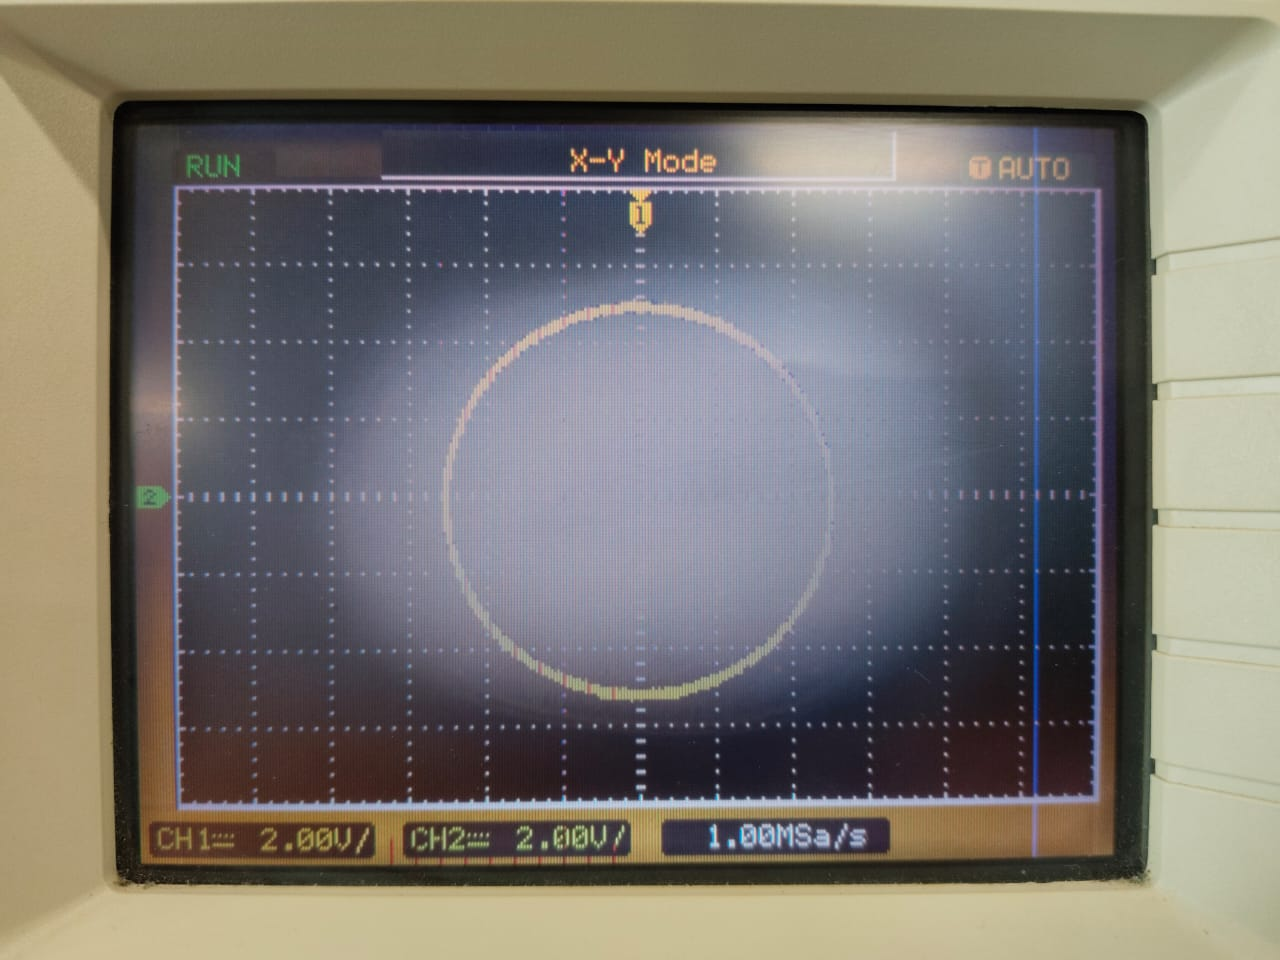
\includegraphics[width=0.5\textwidth]{figs/fig.png}
\label{fig:lissajous}
\end{figure}

\item More complex ratios and phase differences result in intricate patterns.
\item Their symmetry properties depend on the phase shift and amplitude ratios.
\end{itemize}

\section{Applications of Lissajous Figures}
Lissajous figures have applications in various domains, including:
\begin{itemize}
\item \textbf{Oscilloscope Applications:} Used to visualize the phase relationship between two signals.
\item \textbf{Vibration Analysis:} Employed to analyze harmonic motion in mechanical systems.
\item \textbf{Signal Processing:} Used to study frequency components of audio and electrical signals.
\item \textbf{Art and Design:} Generate aesthetically appealing patterns.
\end{itemize}

\section{Analysis of Given Specifications}
Below are various Lissajous figure specifications and their corresponding mathematical solutions.

\subsection{Case 1: $y = \sin(3\text{kHz})$, $x = \sin(5\text{kHz} + 90^\circ)$}

Given:
\[
x(t) = \sin(2\pi \cdot 5000 t + \frac{\pi}{2})
\]
\[
y(t) = \sin(2\pi \cdot 3000 t)
\]

The frequencies are \( \omega_x = 2\pi \cdot 5000 \) and \( \omega_y = 2\pi \cdot 3000 \). The frequency ratio is:
\[
\frac{\omega_x}{\omega_y} = \frac{5000}{3000} = \frac{5}{3}
\]

Since the phase difference is \( 90^\circ = \frac{\pi}{2} \), the figure will be symmetric and display a characteristic pattern with a quarter-period phase shift between the axes.

\subsection{Case 2: $y = \sin(3\text{kHz})$, $x = \sin(4\text{kHz} + 45^\circ)$}

Given:
\[
x(t) = \sin(2\pi \cdot 4000 t + \frac{\pi}{4})
\]
\[
y(t) = \sin(2\pi \cdot 3000 t)
\]

The frequency ratio is:
\[
\frac{\omega_x}{\omega_y} = \frac{4000}{3000} = \frac{4}{3}
\]

The phase difference is \( 45^\circ = \frac{\pi}{4} \), which will result in a more complex Lissajous pattern. The graph will have intricate loops with slight skewing.

\subsection{Case 3: $y = \sin(2\text{kHz} + 45^\circ)$, $x = \sin(3\text{kHz})$}

Given:
\[
x(t) = \sin(2\pi \cdot 3000 t)
\]
\[
y(t) = \sin(2\pi \cdot 2000 t + \frac{\pi}{4})
\]

The frequency ratio is:
\[
\frac{\omega_x}{\omega_y} = \frac{3000}{2000} = \frac{3}{2}
\]

The phase difference of \( 45^\circ \) will result in a skewed Lissajous figure with a diagonal symmetry.

\subsection{Case 4: $y = \sin(1\text{kHz})$, $x = \sin(3\text{kHz} + 45^\circ)$}

Given:
\[
x(t) = \sin(2\pi \cdot 3000 t + \frac{\pi}{4})
\]
\[
y(t) = \sin(2\pi \cdot 1000 t)
\]

The frequency ratio is:
\[
\frac{\omega_x}{\omega_y} = \frac{3000}{1000} = 3
\]

The phase difference of \( 45^\circ \) leads to a figure where the x-axis completes three cycles for every one cycle along the y-axis.

\subsection{Case 5: $y = \sin(1\text{kHz})$, $x = \sin(2\text{kHz} + 45^\circ)$}

Given:
\[
x(t) = \sin(2\pi \cdot 2000 t + \frac{\pi}{4})
\]
\[
y(t) = \sin(2\pi \cdot 1000 t)
\]

The frequency ratio is:
\[
\frac{\omega_x}{\omega_y} = \frac{2000}{1000} = 2
\]

The phase difference of \( 45^\circ \) results in a Lissajous figure with two loops along the x-axis for every loop along the y-axis.

\subsection{Case 6: $y = \sin(1\text{kHz})$, $x = \sin(1\text{kHz})$}

Given:
\[
x(t) = \sin(2\pi \cdot 1000 t)
\]
\[
y(t) = \sin(2\pi \cdot 1000 t)
\]

The frequency ratio is:
\[
\frac{\omega_x}{\omega_y} = \frac{1000}{1000} = 1
\]

Since the frequencies are equal and there is no phase difference (\( 0^\circ \)), the resulting Lissajous figure is a straight line along the diagonal.

\section{Voltage Range}
In all cases, the voltage variation is assumed to be in the range of $[-5, 5]V$.

\section{Conclusion}
Lissajous figures provide an elegant visualization of harmonic motion and phase relationships. Their study offers insights into signal analysis, mechanical vibrations, and artistic designs. Understanding their mathematical properties enhances their practical applications in science and engineering.

\begin{thebibliography}{9}
\bibitem{lissajous} Lissajous, J. A. "On the Study of Vibratory Motion by Means of the Optical Method." Comptes Rendus, 1857.
\bibitem{signal} Smith, S. W. "The Scientist and Engineer's Guide to Digital Signal Processing." California Technical Publishing, 1997.
\end{thebibliography}
\end{document}
